\documentclass[11pt]{article}
\usepackage{mathblatt}
% Tischblatt
% Gesetzt aus aufgaben.jsonl (Prüfstein Musterauftrag, 09.10.2026).
\usepackage{enumitem}
\usetikzlibrary{calc}
\newgeometry{a4paper,margin=18mm,top=15mm,bottom=20mm,footskip=9mm}
\pagestyle{fancy}\fancyhf{}\renewcommand{\headrulewidth}{0pt}
\fancyfoot[L]{\footnotesize\color{mbgrau}Satz des Pythagoras: die Hypotenuse berechnen \textperiodcentered{} Tischblatt}
\fancyfoot[R]{\footnotesize\color{mbgrau}\thepage}
\setlength{\parskip}{3pt}
\renewcommand{\kreuz}[1]{\mbox{$\square$\ #1}\quad}
\newcommand{\kreuzl}[1]{\par\hangindent1.4em\hangafter1\noindent$\square$\ #1}
\newcommand{\marke}[1]{\leavevmode\llap{\scriptsize\color{mbgrau}#1\hspace{9mm}}}
\newcommand{\aufg}[3]{\par\noindent\makebox[0pt][r]{#3}\begin{minipage}[t]{\linewidth}#1\end{minipage}\par}
\newcommand{\aufgg}[4]{\par\noindent\makebox[0pt][r]{#4}\begin{minipage}[t]{0.6\linewidth}\vspace{0pt}#1\end{minipage}\hfill
  \begin{minipage}[t]{0.37\linewidth}\vspace{0pt}\centering #2\end{minipage}\par}
\newcommand{\nr}[1]{\makebox[7mm][l]{\textbf{#1}}}
\begin{document}
\noindent{\Large\bfseries Satz des Pythagoras: die Hypotenuse berechnen}\hfill{\small Name: \rule{40mm}{0.4pt}}\par\smallskip
\noindent{\small\color{mbgrau}Rechne auf einem extra Blatt. Runde, wenn nichts anderes steht, auf eine Stelle nach dem Komma. \emph{Ziel} = Aufgabe am Ende eines Abschnitts.}\par\medskip
\par\Needspace{25mm}\noindent\colorbox{black!12}{\makebox[7mm]{\bfseries\strut A}}\hspace{2mm}{\bfseries Hypotenuse finden und berechnen}\par\smallskip
\aufgg{\hangindent7mm\hangafter1\nr{A1}Das Dreieck liegt anders. Wo ist der rechte Winkel? Berechne die Hypotenuse $x$.}{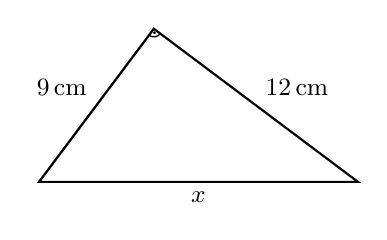
\begin{tikzpicture}[scale=0.27,font=\small]\coordinate (P) at (0,0); \coordinate (Q) at (15,0); \coordinate (R) at (5.4,7.2);\draw[line width=0.8pt] (P) -- (Q) -- (R) -- cycle;\draw[line width=0.5pt] let \p1=($(P)-(R)$), \p2=($(Q)-(R)$), \n1={atan2(\y1,\x1)}, \n2={atan2(\y2,\x2)}, \n3={ifthenelse(mod(\n2-\n1+360,360)<180,\n1,\n2)} in ($(R)+(\n3:0.38)$) arc (\n3:\n3+90:0.38) ($(R)+(\n3+45:0.19)$) circle (0.8pt);\node[above left] at (2.7,3.6) {9\,cm}; \node[above right] at (10.2,3.6) {12\,cm};\node[below] at (7.5,0) {$x$};\end{tikzpicture}}{}{}
\medskip
\aufgg{\hangindent7mm\hangafter1\nr{A2}Die Seiten heißen hier $r$, $s$ und $t$. (a) Schreib die Gleichung des Satzes für dieses Dreieck auf. (b) $r = 8$\,cm, $s = 15$\,cm. Berechne $t$.}{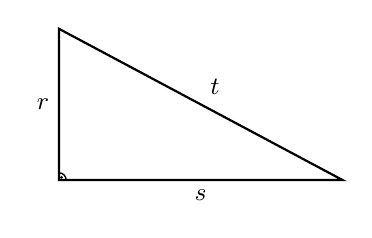
\begin{tikzpicture}[scale=0.24,font=\small]\coordinate (C) at (0,0); \coordinate (B) at (15,0); \coordinate (A) at (0,8);\draw[line width=0.8pt] (A) -- (B) -- (C) -- cycle;\draw[line width=0.5pt] let \p1=($(B)-(C)$), \p2=($(A)-(C)$), \n1={atan2(\y1,\x1)}, \n2={atan2(\y2,\x2)}, \n3={ifthenelse(mod(\n2-\n1+360,360)<180,\n1,\n2)} in ($(C)+(\n3:0.38)$) arc (\n3:\n3+90:0.38) ($(C)+(\n3+45:0.19)$) circle (0.8pt);\node[below] at (7.5,0) {$s$}; \node[left] at (0,4) {$r$};\node[above right] at (7.5,4) {$t$};\end{tikzpicture}}{}{}
\medskip
\aufgg{\hangindent7mm\hangafter1\nr{A3}Welche Gleichung passt zu diesem Dreieck? Kreuze an.\par\smallskip\leftskip7mm \kreuz{$u = v + w$}\ \kreuz{$u = \sqrt{v^2 - w^2}$}\par\kreuz{$u = v^2 + w^2$}\ \kreuz{$u = \sqrt{v^2 + w^2}$}}{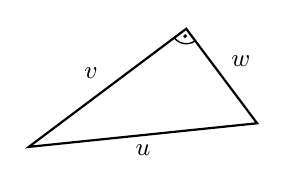
\begin{tikzpicture}[scale=0.5,font=\small]\coordinate (X) at (0,0); \coordinate (Y) at (4,3); \coordinate (Z) at (5.8,0.6);\draw[line width=0.8pt] (X) -- (Y) -- (Z) -- cycle;\draw[line width=0.5pt] let \p1=($(X)-(Y)$), \p2=($(Z)-(Y)$), \n1={atan2(\y1,\x1)}, \n2={atan2(\y2,\x2)}, \n3={ifthenelse(mod(\n2-\n1+360,360)<180,\n1,\n2)} in ($(Y)+(\n3:0.38)$) arc (\n3:\n3+90:0.38) ($(Y)+(\n3+45:0.19)$) circle (0.8pt);\node[above left] at (2,1.5) {$v$}; \node[above right] at (4.9,1.8) {$w$};\node[below] at (2.9,0.3) {$u$};\end{tikzpicture}}{}{}
\medskip
\aufgg{\hangindent7mm\hangafter1\nr{A4}Ein Schrank ist 240\,cm hoch und 70\,cm tief. Er wird liegend zusammengebaut und dann aufgerichtet; dabei kippt er über eine untere Kante. Das Zimmer ist 245\,cm hoch. Geht das? Begründe mit einer Rechnung. Tipp: Welche Strecke der Seitenwand ist am längsten?}{\begin{tikzpicture}[scale=0.62,font=\small]\draw[mbgrau] (-0.3,0) -- (7.4,0); \draw[mbgrau,dashed] (-0.3,4.08) -- (7.4,4.08);\node[above right,font=\scriptsize,mbgrau] at (-0.3,4.08) {Decke: 245\,cm hoch};\draw[line width=0.8pt] (0,0) rectangle (4,1.17);\node[below] at (2,0) {240\,cm}; \node[right] at (4,0.58) {70\,cm};\draw[line width=0.8pt] (6,0) rectangle (7.17,4);\draw[->,mbgrau] (3.2,1.5) to[bend left=35] (5.8,3.0);\node[font=\scriptsize,mbgrau] at (3.4,2.9) {aufrichten};\end{tikzpicture}}{}{{\scriptsize\color{mbgrau}Ziel\hspace{2mm}}}
\medskip
\par\Needspace{25mm}\noindent\colorbox{black!12}{\makebox[7mm]{\bfseries\strut B}}\hspace{2mm}{\bfseries Wenn die Wurzel nicht aufgeht}\par\smallskip
\aufg{\hangindent7mm\hangafter1\nr{B1}Ein rechtwinkliges Dreieck hat die Katheten 5\,cm und 9\,cm. Berechne die Hypotenuse. Runde auf eine Stelle nach dem Komma.}{}{}
\medskip
\aufg{\hangindent7mm\hangafter1\nr{B2}Die Katheten sind 2,5\,m und 4,2\,m lang. Berechne die Hypotenuse auf eine Stelle nach dem Komma.}{}{}
\medskip
\aufg{\hangindent7mm\hangafter1\nr{B3}Die Katheten sind 1,2\,m und 50\,cm lang. Mach zuerst beide Einheiten gleich. Wie lang ist die Hypotenuse?}{}{}
\medskip
\aufgg{\hangindent7mm\hangafter1\nr{B4}Der Bildschirm eines Handys ist 6,5\,cm breit und 14\,cm hoch. Wie lang ist seine Diagonale $d$? Runde auf eine Stelle nach dem Komma.}{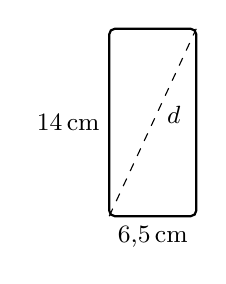
\begin{tikzpicture}[scale=0.17,font=\small]\draw[line width=0.8pt,rounded corners=2pt] (0,0) rectangle (6.5,14);\draw[dashed] (0,0) -- (6.5,14); \node[right] at (3.6,7.6) {$d$};\node[below] at (3.25,0) {6,5\,cm}; \node[left] at (0,7) {14\,cm};\end{tikzpicture}}{}{}
\medskip
\aufg{\hangindent7mm\hangafter1\nr{B5}Ein rechteckiger Park ist 160\,m lang und 70\,m breit. Lena will von einer Ecke zur gegenüberliegenden Ecke. Bisher ging sie außen am Rand entlang. Jetzt gibt es einen geraden Weg quer durch den Park. Wie viele Meter spart sie?}{}{{\scriptsize\color{mbgrau}Ziel\hspace{2mm}}}
\medskip
\par\Needspace{25mm}\noindent\colorbox{black!12}{\makebox[7mm]{\bfseries\strut C}}\hspace{2mm}{\bfseries Sachaufgaben: Leiter, Rampe, Gelände}\par\smallskip
\aufgg{\hangindent7mm\hangafter1\nr{C1}Eine Rampe führt auf eine Stufe. Sie ist waagerecht gemessen 240\,cm lang, die Stufe ist 18\,cm hoch. Wie lang ist die schräge Rampe? Runde auf eine Stelle nach dem Komma.}{\begin{tikzpicture}[scale=0.62,font=\small]\draw[line width=0.8pt] (0,0) -- (5,0) -- (5,0.7) -- cycle;\fill[black!12] (5,0) rectangle (5.8,0.7); \draw (5,0.7) -- (5.8,0.7) -- (5.8,0);\draw[line width=0.5pt] let \p1=($(0,0)-(5,0)$), \p2=($(5,0.7)-(5,0)$), \n1={atan2(\y1,\x1)}, \n2={atan2(\y2,\x2)}, \n3={ifthenelse(mod(\n2-\n1+360,360)<180,\n1,\n2)} in ($(5,0)+(\n3:0.38)$) arc (\n3:\n3+90:0.38) ($(5,0)+(\n3+45:0.19)$) circle (0.8pt);\node[below] at (2.5,0) {240\,cm}; \node[right,font=\scriptsize] at (5.8,0.35) {18\,cm};\node[above left] at (2.5,0.35) {$x$};\node[font=\scriptsize,mbgrau] at (2.6,-0.9) {nicht maßstabsgerecht};\end{tikzpicture}}{}{}
\medskip
\aufgg{\hangindent7mm\hangafter1\nr{C2}Zwischen $A$ und $B$ liegt ein Teich. Man misst über $C$ (rechter Winkel bei $C$): $\overline{CA} = 34$\,m, $\overline{CB} = 12$\,m. Wie weit ist $A$ von $B$ entfernt? Gib auch das Zwischenergebnis $\overline{AB}^{\,2}$ an. Achtung: Welche Seite ist die längste?}{\begin{tikzpicture}[scale=0.8,font=\small]\coordinate (C) at (0,0); \coordinate (A) at (0,3.4); \coordinate (B) at (2.4,0);\fill[black!10,rotate around={-54.8:(1.2,1.7)}] (1.2,1.7) ellipse (0.9 and 0.45);\draw[line width=0.8pt] (A) -- (C) -- (B); \draw[dashed] (A) -- (B);\draw[line width=0.5pt] let \p1=($(B)-(C)$), \p2=($(A)-(C)$), \n1={atan2(\y1,\x1)}, \n2={atan2(\y2,\x2)}, \n3={ifthenelse(mod(\n2-\n1+360,360)<180,\n1,\n2)} in ($(C)+(\n3:0.38)$) arc (\n3:\n3+90:0.38) ($(C)+(\n3+45:0.19)$) circle (0.8pt);\fill (A) circle (1.5pt) node[above] {$A$}; \fill (B) circle (1.5pt) node[right] {$B$};\fill (C) circle (1.5pt) node[below left] {$C$};\node[left] at (0,1.7) {34\,m}; \node[below] at (1.2,0) {12\,m};\node[font=\scriptsize,mbgrau] at (1.25,1.75) {Teich};\end{tikzpicture}}{}{}
\medskip
\aufgg{\hangindent7mm\hangafter1\nr{C3}Ein Fahnenmast wird mit einem Seil gesichert. Das Seil ist in 6\,m Höhe am Mast befestigt und 3\,m vom Mast entfernt im Boden. Für die zwei Knoten braucht man zusätzlich 0,5\,m Seil. Wie lang muss das Seil sein? Runde auf eine Stelle nach dem Komma.}{\begin{tikzpicture}[scale=0.4,font=\small]\draw[line width=0.8pt] (-0.6,0) -- (3.8,0); \draw[line width=1.6pt] (0,0) -- (0,8);\fill[black!25] (0,8) -- (1.6,7.5) -- (0,7) -- cycle;\draw[line width=0.8pt] (0,6) -- (3,0);\draw[line width=0.5pt] let \p1=($(1,0)-(0,0)$), \p2=($(0,1)-(0,0)$), \n1={atan2(\y1,\x1)}, \n2={atan2(\y2,\x2)}, \n3={ifthenelse(mod(\n2-\n1+360,360)<180,\n1,\n2)} in ($(0,0)+(\n3:0.38)$) arc (\n3:\n3+90:0.38) ($(0,0)+(\n3+45:0.19)$) circle (0.8pt);\node[right] at (1.6,3.2) {Seil};\draw[|<->|,mbgrau] (-1.1,0) -- (-1.1,6); \node[left] at (-1.1,3) {6\,m};\node[below] at (1.5,0) {3\,m};\end{tikzpicture}}{}{}
\medskip
\aufg{\hangindent7mm\hangafter1\nr{C4}Herr Kaya will an ein Fenster. Die Unterkante liegt 4,70\,m hoch. Seine Leiter ist 5\,m lang. Wegen eines Beetes muss der Fuß der Leiter 2\,m von der Hauswand entfernt stehen. Reicht die Leiter bis zur Unterkante? Wenn nicht: Um wie viel ist sie zu kurz? Rechne mit zwei Stellen nach dem Komma.}{}{{\scriptsize\color{mbgrau}Ziel\hspace{2mm}}}
\medskip
\par\Needspace{25mm}\noindent\colorbox{black!12}{\makebox[7mm]{\bfseries\strut T}}\hspace{2mm}{\bfseries Probetest}\par\smallskip
\aufg{\hangindent7mm\hangafter1\nr{T1}Welche Aussage ist der Satz des Pythagoras? Kreuze an.\par\smallskip\leftskip7mm \kreuzl{In einem rechtwinkligen Dreieck ist die Hypotenuse so lang wie die beiden Katheten zusammen.}\kreuzl{In einem rechtwinkligen Dreieck ist die Summe der Flächeninhalte der Kathetenquadrate gleich dem Flächeninhalt des Hypotenusenquadrats.}\kreuzl{In einem rechtwinkligen Dreieck liegt dem rechten Winkel eine Kathete gegenüber.}}{}{}
\medskip
\aufgg{\hangindent7mm\hangafter1\nr{T2}Welche Gleichung gilt für dieses Dreieck? Kreuze an.\par\smallskip\leftskip7mm \kreuz{$c^2 = a^2 + b^2$}\ \kreuz{$a^2 = b^2 + c^2$}\par\kreuz{$b^2 = a^2 + c^2$}\ \kreuz{$a = b + c$}}{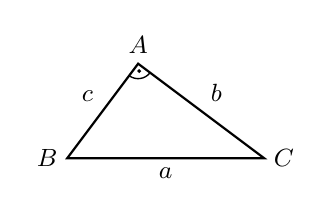
\begin{tikzpicture}[scale=0.5,font=\small]\coordinate (A) at (1.8,2.4); \coordinate (B) at (0,0); \coordinate (C) at (5,0);\draw[line width=0.8pt] (A) -- (B) -- (C) -- cycle;\draw[line width=0.5pt] let \p1=($(B)-(A)$), \p2=($(C)-(A)$), \n1={atan2(\y1,\x1)}, \n2={atan2(\y2,\x2)}, \n3={ifthenelse(mod(\n2-\n1+360,360)<180,\n1,\n2)} in ($(A)+(\n3:0.38)$) arc (\n3:\n3+90:0.38) ($(A)+(\n3+45:0.19)$) circle (0.8pt);\node[above] at (A) {$A$}; \node[left] at (B) {$B$}; \node[right] at (C) {$C$};\node[below] at (2.5,0) {$a$}; \node[above right] at (3.4,1.2) {$b$};\node[above left] at (0.9,1.2) {$c$};\end{tikzpicture}}{}{}
\medskip
\aufg{\hangindent7mm\hangafter1\nr{T3}Ein Fußballfeld ist 105\,m lang und 68\,m breit. Ein Spieler läuft auf gerader Linie von einer Eckfahne zur gegenüberliegenden. Wie lang ist sein Weg? Gib das Zwischenergebnis an und runde auf eine Stelle nach dem Komma.}{}{}
\medskip
\aufg{\hangindent7mm\hangafter1\nr{T4}Familie Berg zieht um. Eine Gardinenstange ist 2,60\,m lang. Der Boden des Laderaums im Transporter ist 2,20\,m lang und 1,30\,m breit. Kann die Stange flach auf dem Boden liegen? Begründe mit einer Rechnung.}{}{{\scriptsize\color{mbgrau}Ziel\hspace{2mm}}}
\medskip
\end{document}
